%!TEX TS-program = xelatex
%!TEX encoding = UTF-8 Unicode

\documentclass[12pt]{extarticle}
% extarticle is like article but can handle 8pt, 9pt, 10pt, 11pt, 12pt, 14pt, 17pt, and 20pt text

\def \ititle {Origins of Mind}
 
\def \isubtitle {Lecture 02}
 
\def \iauthor {Stephen A. Butterfill}
\def \iemail{s.butterfill@warwick.ac.uk}
\date{}

%for strikethrough
\usepackage[normalem]{ulem}

\input{$HOME/Documents/submissions/preamble_steve_handout}

%\bibpunct{}{}{,}{s}{}{,}  %use superscript TICS style bib
%remove hanging indent for TICS style bib
%TODO doesnt work
\setlength{\bibhang}{0em}
%\setlength{\bibsep}{0.5em}


%itemize bullet should be dash
\renewcommand{\labelitemi}{$-$}

\begin{document}

\begin{multicols}{3}

\setlength\footnotesep{1em}


\bibliographystyle{newapa} %apalike

%\maketitle
%\tableofcontents




%--------------- 
%--- start paste


\def \ititle {Origins of Mind}
 
\def \isubtitle {Lecture 02}
 
 
 
\
 
 
 
\begin{center}
 
{\Large
 
\textbf{\ititle}: \isubtitle
 
}
 
 
 
\iemail %
 
\end{center}
 
 
 
\section{Categorical Perception of Colour}
 
What is categorical perception of colour commonly taken to explain?
The diagram below represents sequences of three colours.
The vertical sequence shows three greens and the uppermost horizontal sequence shows a blue, a purple and a pink.
\begin{center}
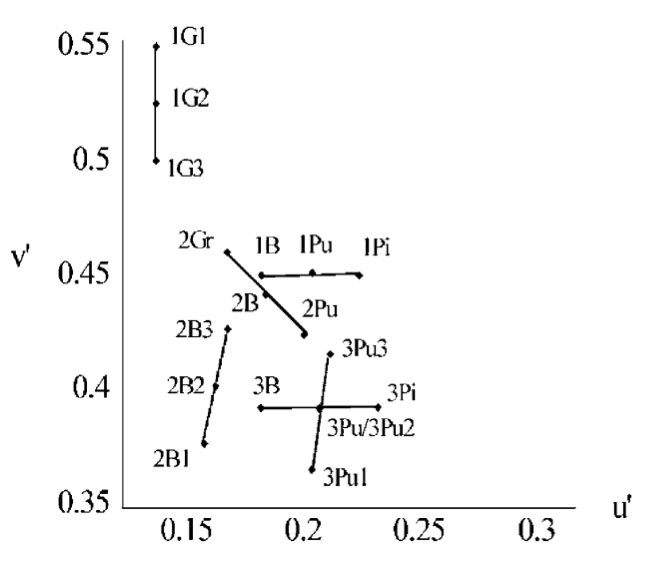
\includegraphics[scale=0.3]{daoutis_2006_fig_A1.png}
\end{center}
\begin{center} \citealp{Daoutis:2006ij} figure A1 \end{center}
 
Each colour differs from its neighbours by the same amount according to a standard measure based on the human eye's abilities to discriminate wavelengths.
 
Yet the greens are often judged to look quite similar and the blue-pink-purple to look very different \citep[p.\ 12--7]{Roberson:1999rk}.
When people are asked to name these colours, they often give the same name to the greens but different names to members of the blue-pink-purple sequence.
And people are generally faster and more accurate in discriminating between members of the blue-pink-purple sequence than members of the green sequence (faster: \citealp{Bornstein:1984cb}; more accurate: \citealp[p.\ 22--7]{Roberson:1999rk}).
 
\textbf{pop-out} ‘Such targets pop out of the display, so that the time it takes to find them is independent of the number of distractors’ \citep[p.\ 117]{Treisman:1986pm}.
 
When target and distractors differ in colour category there can be pop-out effects \citep{Daoutis:2006qk}.
 
A process is \emph{automatic} just if
whether it happens is independent of the subject’s task and motivation (to a significant degree)
 
vMMN (visual mismatch negativity): an event-related potential thought to index pre-attentive change detection in the visual cortex

 
 
 
\section{Categorical Perception in Infancy}
 
Categorical perception of colour emerges early in infancy. This has been demonstrated with four-month-olds using habituation \citep{Bornstein:1976of} and visual search \citep{Franklin:2005xk}.
 
Slightly older infants can make use of colour properties such as red and green to recognise objects.
 
For instance, nine-months-olds can determine whether an object they saw earlier is the same as a subsequently presented object on the basis of its colour \citep{Wilcox:2008jk}.
 
By the time they are two years old, toddlers who do not comprehend any colour words can use colour categories implicitly in learning and using proper names; for instance, they are able to learn and use proper names for toy dinosaurs that differ only in colour \citep[][Experiment 3]{Soja:1994np}.
 
So infants and toddlers enjoy categorical perception of colour and may benefit from it in recognising and learning about objects.
 
However children only acquire concepts of, and words for, colours some time later; and colour concepts, like colour words, are acquired gradually \citep{Pitchford:2005hm,Kowalski:2006hk,Sandhofer:1999if,Sandhofer:2006qo}.
 
\subsection{Other cases}
 
Infants enjoy categorical perception not only of colour but also of orientation \citep{franklin:2010_hemispheric}, speech \citep{Kuhl:1987la,Kuhl:2004nv,Jusczyk:1995it} and facial expressions of emotion \citep{Etcoff:1992zd,Kotsoni:2001ph,Campanella:2002aa}.
 
 
 
\section{Categorical Perception and Knowledge}
 
Categorical perception provides ‘the building blocks—the elementary units—for higher-order categories’
\citep[p.\ 3]{Harnad:1987ej}.
 
‘The module … automatically provides a conceptual identification of its input for central thought … in exactly the right format for inferential processes’
\citep[pp.\ 193--4]{Leslie:1988ct}
 
Acquiring colour concepts depends on acquiring colour words
\citep{Kowalski:2006hk}.
 
‘the course of acquisition for color is protracted and errorful’
\citep{Sandhofer:2006qo}
 
‘the earliest conceptual functioning consists of a redescription of perceptual structure’
\citep{Mandler:1992vn}
 
Colour words shape adults’ categorical perception \citep{Roberson:2007wg,Winawer:2007im}.
 
Categorical perception provides ‘the building blocks—the elementary units—for higher-order categories’
\citep[p.\ 3]{Harnad:1987ej}.
 
 
 
\section{Categorical Perception in Infants and Adults}
 
In adults, categorical perception of colour disappears in the face of predictable verbal interference but not non-verbal interference
\citep{Roberson:2000ge,Pilling:2003bi,Wiggett:2008xt}.
 
‘surprising it would be indeed if I have a perceptual experience as of red because I call the perceived object ‘red’’
\citep[pp.\ 324--5]{Stokes:2006fd}
 
There is evidence that the infant mode of categorical perception of colour continues to operate in adults, although it is often inhibited or overshadowed by the adult mode \citep{Gilbert:2006yb}.
 


 

%--- end paste
%--------------- 
 
\footnotesize 
\bibliography{$HOME/endnote/phd_biblio}

\end{multicols}

\end{document}